\documentclass{article}
\usepackage[utf8]{inputenc}

\title{MATH2710 — Portfolio 7.3}
\author{Mike Medved}
\date{March 23rd, 2023}

\usepackage{color}
\usepackage{amsthm}
\usepackage{amssymb} 
\usepackage{amsmath}
\usepackage{lmodern}
\usepackage{mathtools, nccmath}
\usepackage{listings}
\usepackage[margin=1in]{geometry} 
\usepackage[table,xdraw,dvipsnames]{xcolor}
\usepackage{tikz}
\usepackage{pgfplots}
\usepackage{graphicx}
\usepackage{xparse}
\usepackage{multicol}
%
\DeclarePairedDelimiterX{\set}[1]{\{}{\}}{\setargs{#1}}
\NewDocumentCommand{\setargs}{>{\SplitArgument{1}{;}}m}
{\setargsaux#1}
\NewDocumentCommand{\setargsaux}{mm}
{\IfNoValueTF{#2}{#1} {#1\,\delimsize|\,\mathopen{}#2}}%{#1\:;\:#2}

\parindent = 0pt

\newtheorem*{thm}{Theorem}

\begin{document}

\maketitle

\section*{Existence/Uniqueness}

\subsection*{Outline of Existence Proof}

An existence proof uses any method to show that a solution exists such that $\exists x \in X, P(x)$.

\subsection*{Outline of Existence + Uniqueness Proof}

In the case of an existence + uniqueness proof, you must first prove that $\exists x \in X, P(x)$ using any method, and then prove that $x$ is a unique solution for the given statement.

\subsection*{Proof Examples}

\begin{enumerate}
    \item Prove that $\exists x \in \mathbb{R}, x^2-6x+8=0$.
    \item Prove that $\exists! x \in \mathbb{R}, 5x-15=0$.
    \item Prove that $\exists p \in \text{Primes}$, such that $p+8$ is also a prime number.
    \item Prove that $\exists f \text{ differentiable function}$ on real interval $I$, such that $f = f'$ on $I$.
    \item Prove that if a function $f$ is not one-to-one on the real internal $I$, then $f$ is not strictly increasing.
    \item Let $S = \left\{a\sqrt{7} + b; (a,b) \in \mathbb{Z}\right\}$, prove that $\forall x \in S$, there exists uniquely $(a, b) \in \mathbb{Z}$ such that $x = a\sqrt{7}+b$.
\end{enumerate}

\subsubsection*{Example 1.}

We can use the quadratic formula to solve for $x$ in this case. The quadratic formula is $x = \frac{-b \pm \sqrt{b^2-4ac}}{2a}$, where $a = 1$, $b = -6$, and $c = 8$. This gives us $x = \frac{6 \pm \sqrt{6^2-4(1)(8)}}{2(1)} = \frac{6 \pm \sqrt{36-32}}{2} = \frac{6 \pm \sqrt{4}}{2} = \frac{6 \pm 2}{2} = 4 \pm 1$. Since $x$ is a real number, we can conclude that $\exists x \in \mathbb{R}, x^2-6x+8=0$.

\subsubsection*{Example 2.}

Firstly, we must show that there exists an $x$ such that $5x-15=0$. In this case, we can algebraically solve the equation to find $x=3$. Now, we must show that $x$ is a unique solution. In order to do this, we must show that $5x-15=0$ is not true for any other $x$. In this case, we can show that $5x-15=0$ is not true for any other $x$ by showing supposing there are $x_1, x_2$ such that $5x_1-15=0$ and $5x_2-15=0$. Then, we can show that $x_1=x_2$ by dividing by $5$ for each equation, and then isolating $x_1$ and $x_2$ on each side of the equation. This gives us $x_1 = \frac{15}{5} = 3$ and $x_2 = \frac{15}{5} = 3$, so $x_1=x_2$. Therefore, we can conclude that $\exists! x \in \mathbb{R}, 5x-15=0$. 

\subsubsection*{Example 3.}

Let's use $p = 3$, thus $p + 8 = 11$. In this case, both $p, p+8$ are primes. Thus, $\exists p \in \text{ Primes }$, such that $p+8$ is also a prime number.

\subsubsection*{Example 4.}

Consider $f(x)=ce^x$ for some $c \in \mathbb{R}$. We can differentiate $f(x)$ to obtain $f'(x)=ce^x$. In this case $f(x)=f'(x)$ when iff $c=1$, thus we can conclude that $\exists f \text{ differentiable function}$ on real interval $I$, such that $f = f'$ on $I$. 

\subsubsection*{Example 5.}

Assume that $f$ is one-to-one on the real interval $I$, we aim to prove that $f$ is strictly increasing. That is, the following: $x_1 \neq x_2 \Rightarrow f(x_1) \neq f(x_2)$.

$\hfill \break$
Let $x_1, x_2$ be $x_1 \neq x_2$, to prove: $f(x_1) \neq f(x_2)$. Without loss of generality, let's assume $x_1 < x_2$. As $f$ is strictly increasing, we have $f(x_1) < f(x_2)$. Hence $f(x_1) \neq f(x_2)$.

\subsubsection*{Example 6.}

\textbf{Existence Proof:} 
\begin{proof}
    As $x \in S$, by definition $\exists(a,b) \in \mathbb{Q}, x = a \cdot \sqrt{7} + b.$
\end{proof}

\textbf{Uniqueness Proof:}
\begin{proof}
    Assume absurdly that $\exists((a_1, b_1), (a_2, b_2))$ couples of rational numbers, such that:

    \begin{equation*}
        \begin{cases}
            x = a_1 \cdot \sqrt{7} + b_1 \hspace{0.5cm} \text{(1)}\\
            x = a_2 \cdot \sqrt{7} + b_2 \hspace{0.5cm} \text{(2)} \\
            (a_1, b_1) \neq (a_2, b_2) \hspace{0.35cm} \text{(3)}
        \end{cases}
    \end{equation*}

    By (1) and (2), we can see that:
    \begin{align*}
        a_1 \cdot \sqrt{7} + b_1 &= a_2 \cdot \sqrt{7} + b_2 \\
        a_1 \cdot \sqrt{7} - a_2 \cdot \sqrt{7} &= b_2 - b_1 \\
        (a_1 - a_2) \cdot \sqrt{7} &= b_2 - b_1
    \end{align*}

    Thus, we can now check for the two cases wherein $a_1 - a_2$ is equal to zero or not.

    $\hfill \break$
    \textbf{Case 1. $a_1 - a_2 \neq 0$}
    $\hfill \break$
    $\sqrt{2} = \frac{b_2-b_1}{a_1-a_2} \Rightarrow \sqrt{2} \in \mathbb{Q}$. The fact that $\sqrt{2} \in \mathbb{Q}$ is a contradiction.
    
    $\hfill \break$
    \textbf{Case 2. $a_1 - a_2 = 0$}
    $\hfill \break$
    As $a_1-a_2=0$, we have that $b_2-b_1=0$, so $b_1=b_2$ and since $a_1-a_2=0$ the same logic applies. This is a contradiction with respect to  statement (3).
\end{proof}

\subsection*{Min-Max Theorem}

If $f$ is continuous on $[a,b]$, then $\exists M, m \in [a,b]$ such that $f(M) \geq f(m) \forall x \in [a,b]$ and $f(m) \leq f(M) \forall x \in [a,b]$.

\begin{figure}[!htb]
    \centering
    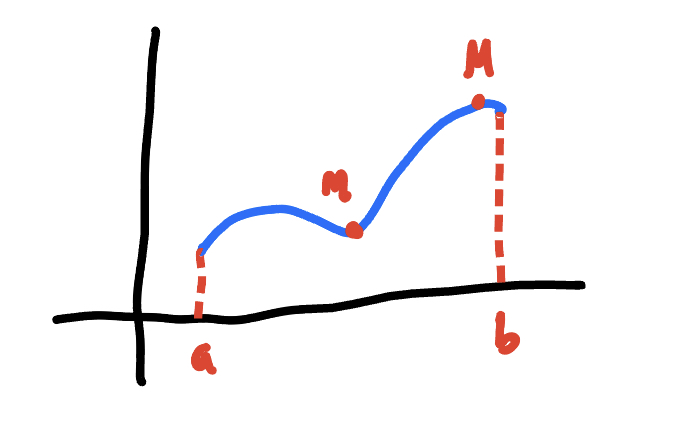
\includegraphics[scale=0.15]{min-max-theorem.jpeg}
    \caption{Visualization of The Min-Max Theorem}
    \label{fig:min-max-theorem}
\end{figure}

\newpage
\subsubsection*{Example}

An example of when the Min-Max Theorem fails to hold is when $f(x) = x^2$ on $[-1,1]$. In this case, $f(-1) = 1$ and $f(1) = 1$, so $f(-1) \leq f(x) \leq f(1)$ for all $x \in [-1,1]$, but $f(x) = 0$ has no solution in $[-1,1]$.

\begin{figure}[!htb]
    \centering
    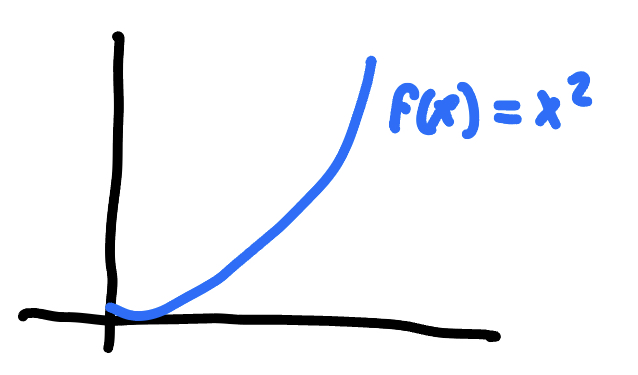
\includegraphics[scale=0.15]{min-max-theorem-fail.jpeg}
    \caption{Visualization of The Min-Max Theorem Failing for $f(x) = x^2$}
    \label{fig:min-max-theorem-fail}
\end{figure}

\subsection*{Rolle's Theorem}

If $f$ is continuous on $[a,b]$, differentiable on $(a,b)$, and $f(a) = f(b)$, then $\exists c \in (a,b)$ such that $f'(c) = 0$.

\begin{figure}[!htb]
    \centering
    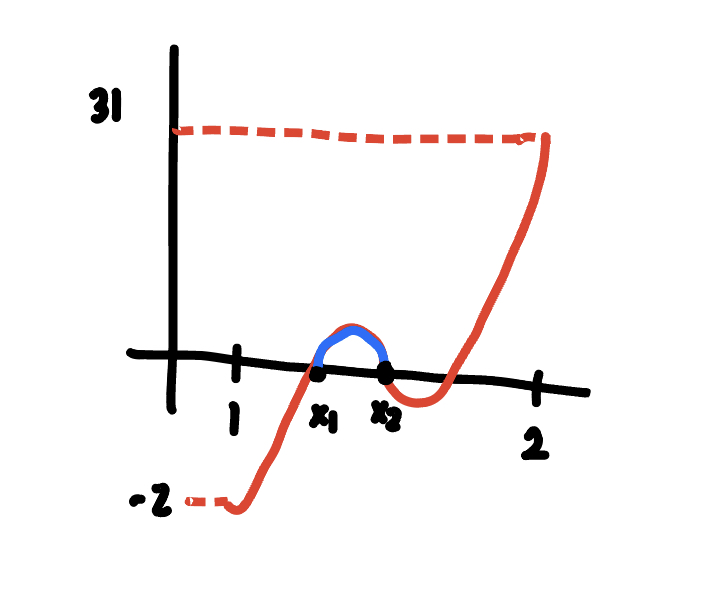
\includegraphics[scale=0.20]{rolles-theorem.jpeg}
    \caption{Visualization of Rolle's Theorem}
    \label{fig:rolles-theorem}
\end{figure}

In order to accomplish this proof, there are several major theorems utilized. These are the Min-Max Theorem, Fermat's Theorem, One-To-One Property, and the Intermediate Value Theorem.

\subsubsection*{Components of Rolle's Theorem}

The hypothesis of Rolle's Theorem is proved using an existence proof, and the conclusion is proved using a uniqueness proof. This is because the hypothesis is that $\exists c \in (a,b)$ such that $f'(c) = 0$, and the conclusion is that $c$ is unique.

\subsubsection*{Cases}

There are two cases that must be proved in order to prove Rolle's Theorem. The first case is when $f$ is constant on $[a,b]$, and the second case is when $f$ is not constant on $[a,b]$.

\begin{figure}[!htb]
    \centering
    \begin{minipage}{0.45\textwidth}
        \centering
        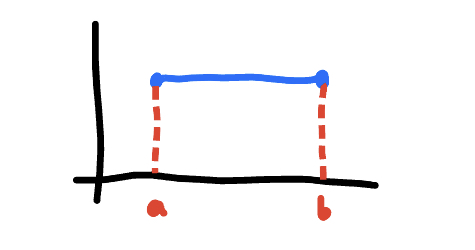
\includegraphics[scale=0.25]{rolles-theorem-case-a.jpeg}
        \caption{Constant Case}
        \label{fig:rolles-theorem-case-a}
    \end{minipage}\hfill
    \begin{minipage}{0.45\textwidth}
        \centering
        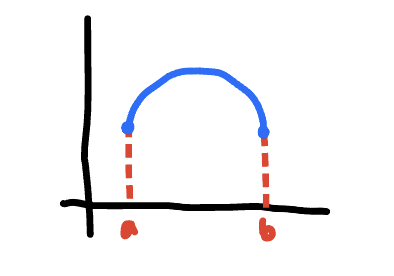
\includegraphics[scale=0.25]{rolles-theorem-case-b.jpeg}
        \caption{Non-Constant Case}
        \label{fig:rolles-theorem-case-b}
    \end{minipage}
\end{figure}

\subsection*{Strictly Increasing Functions}

If $f$ is strictly increasing on the real interval $I$, then $f$ must be one-to-one on $I$. This means that both:

\begin{enumerate}
    \item \textbf{Strictly Increasing:} Let $x_1, x_2 \in I, x_1 < x_2 \Rightarrow f(x_1) < f(x_2), \forall (x_i, x_j) \in I$.
    \item \textbf{One-to-One:} Let $x_1, x_2 \in I, x_1 \neq x_2 \Rightarrow f(x_1) \neq f(x_2), \forall (x_i, x_j) \in I$.
\end{enumerate}

A visual example of a strictly increasing function is $f(x) = x^2$, shown below:

\begin{figure}[!htb]
    \centering
    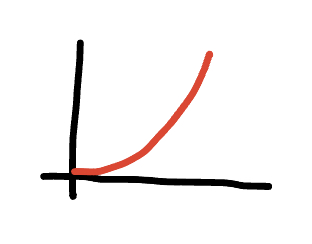
\includegraphics[scale=0.25]{strictly-increasing.jpeg}
    \caption{Example of a Strictly Increasing Function}
    \label{fig:strictly-increasing-function}
\end{figure}

\subsection*{One-To-One Property}

A function being one-to-mean means that no two x-values can have the same y-value. Let $x_1, x_2 \in I, x_1 \neq x_2 \Rightarrow f(x_1) \neq f(x_2), \forall (x_i, x_j) \in I$.

$\hfill \break$
An example of a function that is \textit{not} one-to-one, is $f(x) = (x-2)^2$. This is because $\forall x \in I, f(x)$ is not unique.

\begin{figure}[!htb]
    \centering
    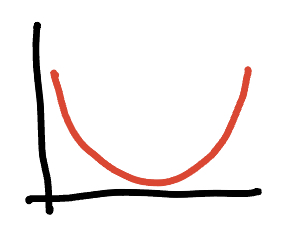
\includegraphics[scale=0.25]{not-one-to-one.jpeg}
    \caption{Example of a Function that is Not One-To-One}
    \label{fig:one-to-one}
\end{figure}

\subsection*{Proof of One-to-One Property}

\begin{thm}
    We aim to show that $f$ is one-to-one on the real interval $I$.
\end{thm}

\begin{proof}
    To be one-to-one means that $\forall (x_1, x_2), x_1 \neq x_2 \Rightarrow f(x_1) \neq f(x_2)$. 
    
    $\hfill \break$
    Let $x_1, x_2$ be $x_1 \neq x_2$, we aim to prove that $f(x_1) \neq f(x_2)$. Thus, without loss of generality, let $x_1 < x_2$. As $f$ is strictly increasing in this case, we have that $f(x_1) < f(x_2)$, and thus $f(x_1) \neq f(x_2) \forall (x_1, x_2) \in I$.
\end{proof}

\newpage
\subsection*{Intermediate Value Property}

Let $f$ be a continuous function on $[a,b]$, then $\forall \lambda \in (f(a), f(b)), \exists c \in (a,b)$ such that $f'(c) = \lambda$.

This is shown below in the following figure.

\begin{figure}[!htb]
    \centering
    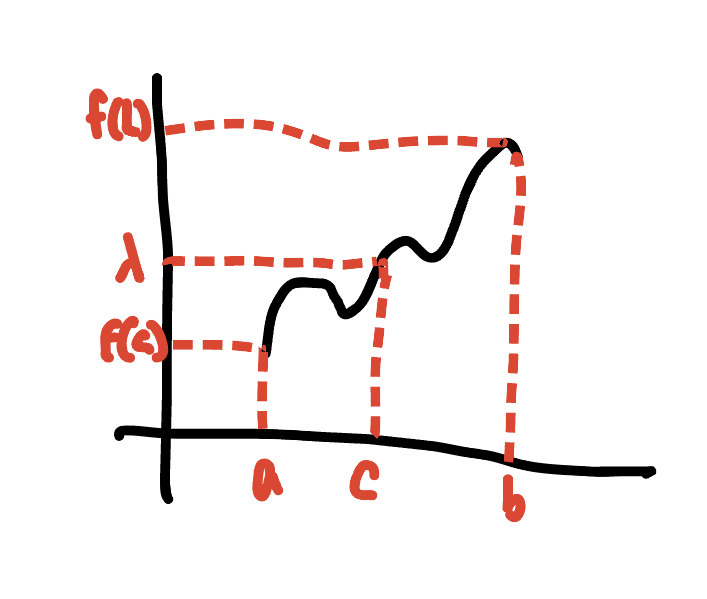
\includegraphics[scale=0.25]{intermediate-val-thm.jpeg}
    \caption{Visualization of the Intermediate Value Theorem}
    \label{fig:intermediate-value-theorem}
\end{figure}

\end{document}